%____________________________________________________________________________||
\section{Corrections to cross section for SM samples}
\label{sec:sideband_corrections}
The cross sections for the most relevant SM background are summarised in Table~\ref{tab:cross_sections_bkg}.

\begin{table}[!h]
  \scriptsize
  \centering
  \topcaption{Cross sections for the main SM backgrounds.}
  \label{tab:cross_sections_bkg}
  \begin{tabular}
    {c|c|c|c}
    \hline\hline
    \textbf{Sample} & \textbf{Cross section (pb)} & \textbf{Accuracy} & \textbf{K-factor} \\
    \hline
    W+jets, $100 < \scalht < 200$ GeV & $1347 \pm 2$ & LO & 1.21 \\
    W+jets, $200 < \scalht < 400$ GeV & $360 \pm 1$ & LO & 1.21 \\
    W+jets, $400 < \scalht < 600$ GeV & $48.9 \pm 0.17$ & LO & 1.21 \\
    W+jets, $600 < \scalht < 800$ GeV & $12.8 \pm 0.4$ & LO & 1.21 \\
    W+jets, $800 < \scalht < 1200$ GeV & $5.26 \pm 0.19$ & LO & 1.21 \\
    W+jets, $1200 < \scalht < 2500$ GeV & $1.33 \pm 0.05$ & LO & 1.21 \\
    W+jets, $\scalht > 2500$ GeV & $0.0309 \pm 0.0011$ & LO & 1.21 \\
    \hline
    DY+jets, $100 < \scalht < 200$ GeV & $139 \pm 4$ & LO & 1.23 \\
    DY+jets, $200 < \scalht < 400$ GeV & $42.8 \pm 1.4$ & LO & 1.23 \\
    DY+jets, $400 < \scalht < 600$ GeV & $5.5 \pm 0.2$ & LO & 1.23 \\
    DY+jets, $\scalht > 600$ GeV & $2.2 \pm 0.8$ & LO & 1.23 \\
    \hline
    $\gamma$+jets, $40 < \scalht < 100$ GeV & $20730 \pm 66$ & LO & - \\
    $\gamma$+jets, $100 < \scalht < 200$ GeV & $9226 \pm 36$ & LO & - \\
    $\gamma$+jets, $200 < \scalht < 400$ GeV & $2281 \pm 47$ & LO & - \\
    $\gamma$+jets, $400 < \scalht < 600$ GeV & $273 \pm 9$ & LO & - \\
    $\gamma$+jets, $\scalht > 600$ GeV & $94.5 \pm 3.2$ & LO & - \\
    \hline
    $Z\rightarrow \nu\nu$+jets, $100 < \scalht < 200$ GeV & $280.47$ & LO & 1.23 \\
    $Z\rightarrow \nu\nu$+jets, $200 < \scalht < 400$ GeV & $78.36$ & LO & 1.23 \\
    $Z\rightarrow \nu\nu$+jets, $400 < \scalht < 600$ GeV & $10.94$ & LO & 1.23 \\
    $Z\rightarrow \nu\nu$+jets, $\scalht > 600$ GeV & $4.20$ & LO & 1.23 \\
    \hline
    TTJets & $831.76^{+20}_{-30}$ & NNLO & - \\    
    \hline \hline
  \end{tabular}
\end{table}


In the high-\scalht, high-\etmiss corner of the phase space used in this search, the normalisations of the MC samples do not necessarily agree with the observation. 
Moreover, the cross section is known only to a limited number of perturbative orders and additional corrections could be in principle sizeable. \\
Nonetheless, the analysis strategy for the background predictions is built in such a way to be mildly, if not negligibly, dependent on these corrections. 
The backgrounds are in fact estimated from control regions in data, and the effect of cross section corrections on the transfer factors is expected to largely cancel out, 
because the background composition is very similar between the signal region and the control regions used to estimate each background. \\
However, the effect could be sizeable for the closure test procedure described in Sec.~\ref{sec:bkgdnorm-syst}, because in this case much more ``extreme'' translations are done. 
For instance, the test carried on in the single muon control sample, where events with no b-tags are used to predict events with 1 b-tag maps 
a $W$-enriched sample to a $t\bar{t}$-enriched one and is sensitive to the relative corrections of $W$ with respect to $t\bar{t}$. 
For this reason it's important to measure any residual cross section corrections. This is done using sidebands in data enriched in a specific process, as described in the following. 

\subsection{Correction to the $\gamma$+jets sample}
\label{sec:sideband_corrections_gjets}
The situation is somehow different for $\gamma$+jets with respect to the other processes. 
In fact the cross section for this process is known only at LO and no $k$-factor has been calculated yet for 13 TeV, 
so a worse agreement is expected for the yields in the single photon control region.
The observation confirms indeed this hypothesis, with the simulation underestimating the yields by $\sim 20\%$. \\
A correction is derived using a sideband in data, by selecting events in the region $350 < \scalht < 400$ GeV. 
The data yields are corrected for the small QCD contamination (taken from MC) and divided by the expected number of events in the simulation. 
The sideband is shown in Fig.~\ref{fig:gjets_HTsideband} (left).
The correction factor to be applied to the GJets sample found with this procedure is $1.30 \pm 0.08$, 
which is in fair agreement with the $k-$factor used in the 8 TeV analysis ($\sim 1.21$). 

\begin{figure}[!h]
  \centering
  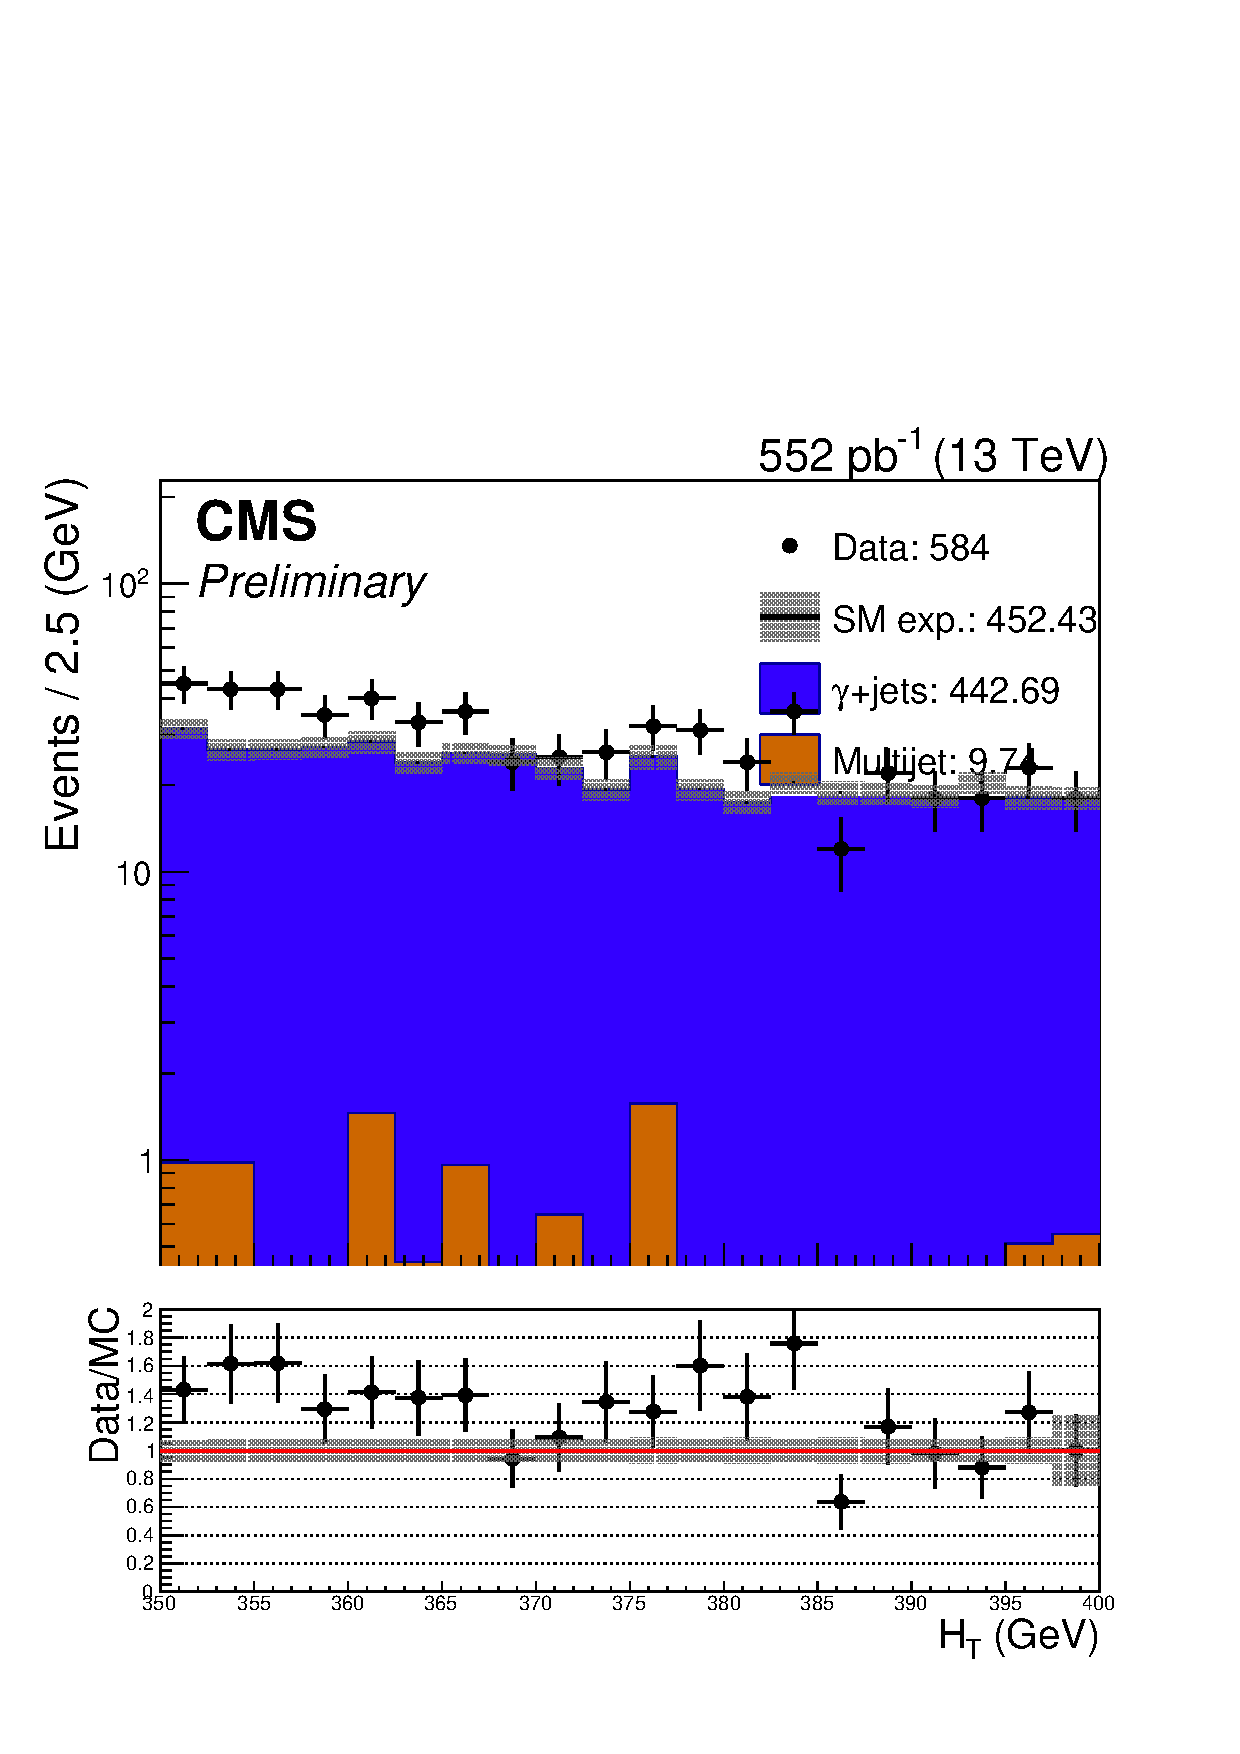
\includegraphics[width=0.45\textwidth]{figures/sidebandCorr/htSideband_NMinusOne_HT_GJets}
  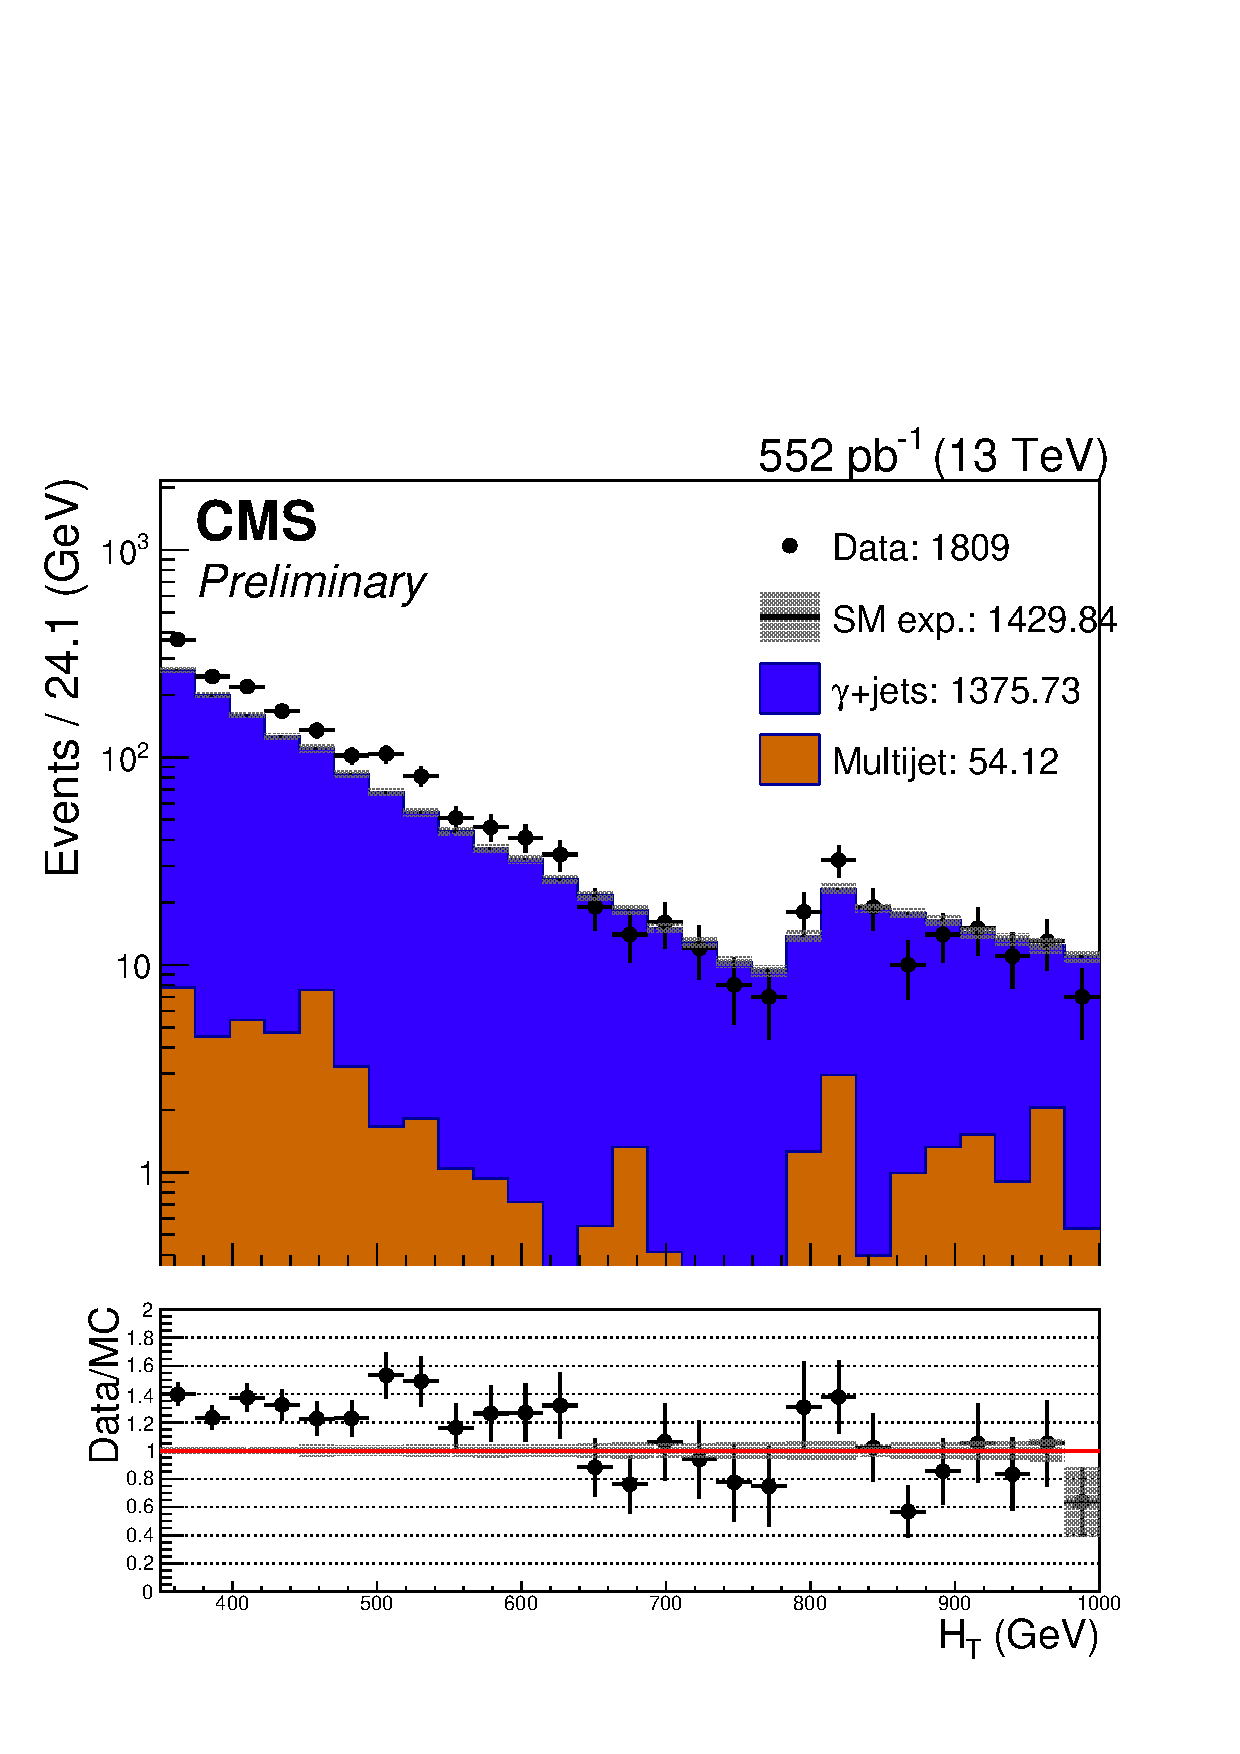
\includegraphics[width=0.45\textwidth]{figures/sidebandCorr/ht_NMinusOne_HT_GJets}
  \caption{The single photon events compared to the MC expectation in the sideband $350 < \scalht < 400$ GeV (left) and in the full \scalht range (right)}
  \label{fig:gjets_HTsideband}
\end{figure}



\subsection{Correction to the $W$+jets, $t\bar{t}$+jets and $Z$+jets samples}
\label{sec:sideband_corrections_w_z_tt}
For the $W$+jets, $t\bar{t}$+jets and $Z$+jets samples we expect smaller corrections, because the cross section is known 
with better accuracy, either by complete calculation or via $k$-factors applied to the LO cross section. 
For this reason, the use of a sideband in \scalht is not optimal in this case, since it is more sensitive to the modelling 
of the \scalht shape in the LO MC samples (we plan to cross-check with NLO samples in the future). 
The low-\scalht sideband is suboptimal in particular for $t\bar{t}$, because 
it selects events with a rare topology for this kind of process, which comes with larger jet multiplicities and thus large value of \scalht. \\
Instead, the $\mhtmet > 1.25$ sideband is used, with the following selection:
\begin{itemize}
\item \wj: single muon, $\nj = 2,3$, $\nb = 0$
\item \zj: double muon, $\nj = 2,3$, $\nb = 0$
\item \ttj: single muon, $\nj \geq 2$, $\nb \geq 2$
\end{itemize}

These selections give a purity of 78\%, 96\% and 92\% respectively for \wj, \zj and \ttj. All contaminations are estimated from MC.\\
The \mhtmet distributions for these three selection are shown in Fig.~\ref{fig:w_z_tt_MHTOverMETsideband}. \\
These distributions are not very well modelled by the simulation, pointing to possible reconstruction effects not yet understood in this first stage of data commissioning. 
The \ttj enriched distribution (right) also confirms the effect of missing b-tag scale factors, whose effect is also seen in the \nb  distribution. %FIXME: add reference!  

\begin{figure}[!h]
  \centering
  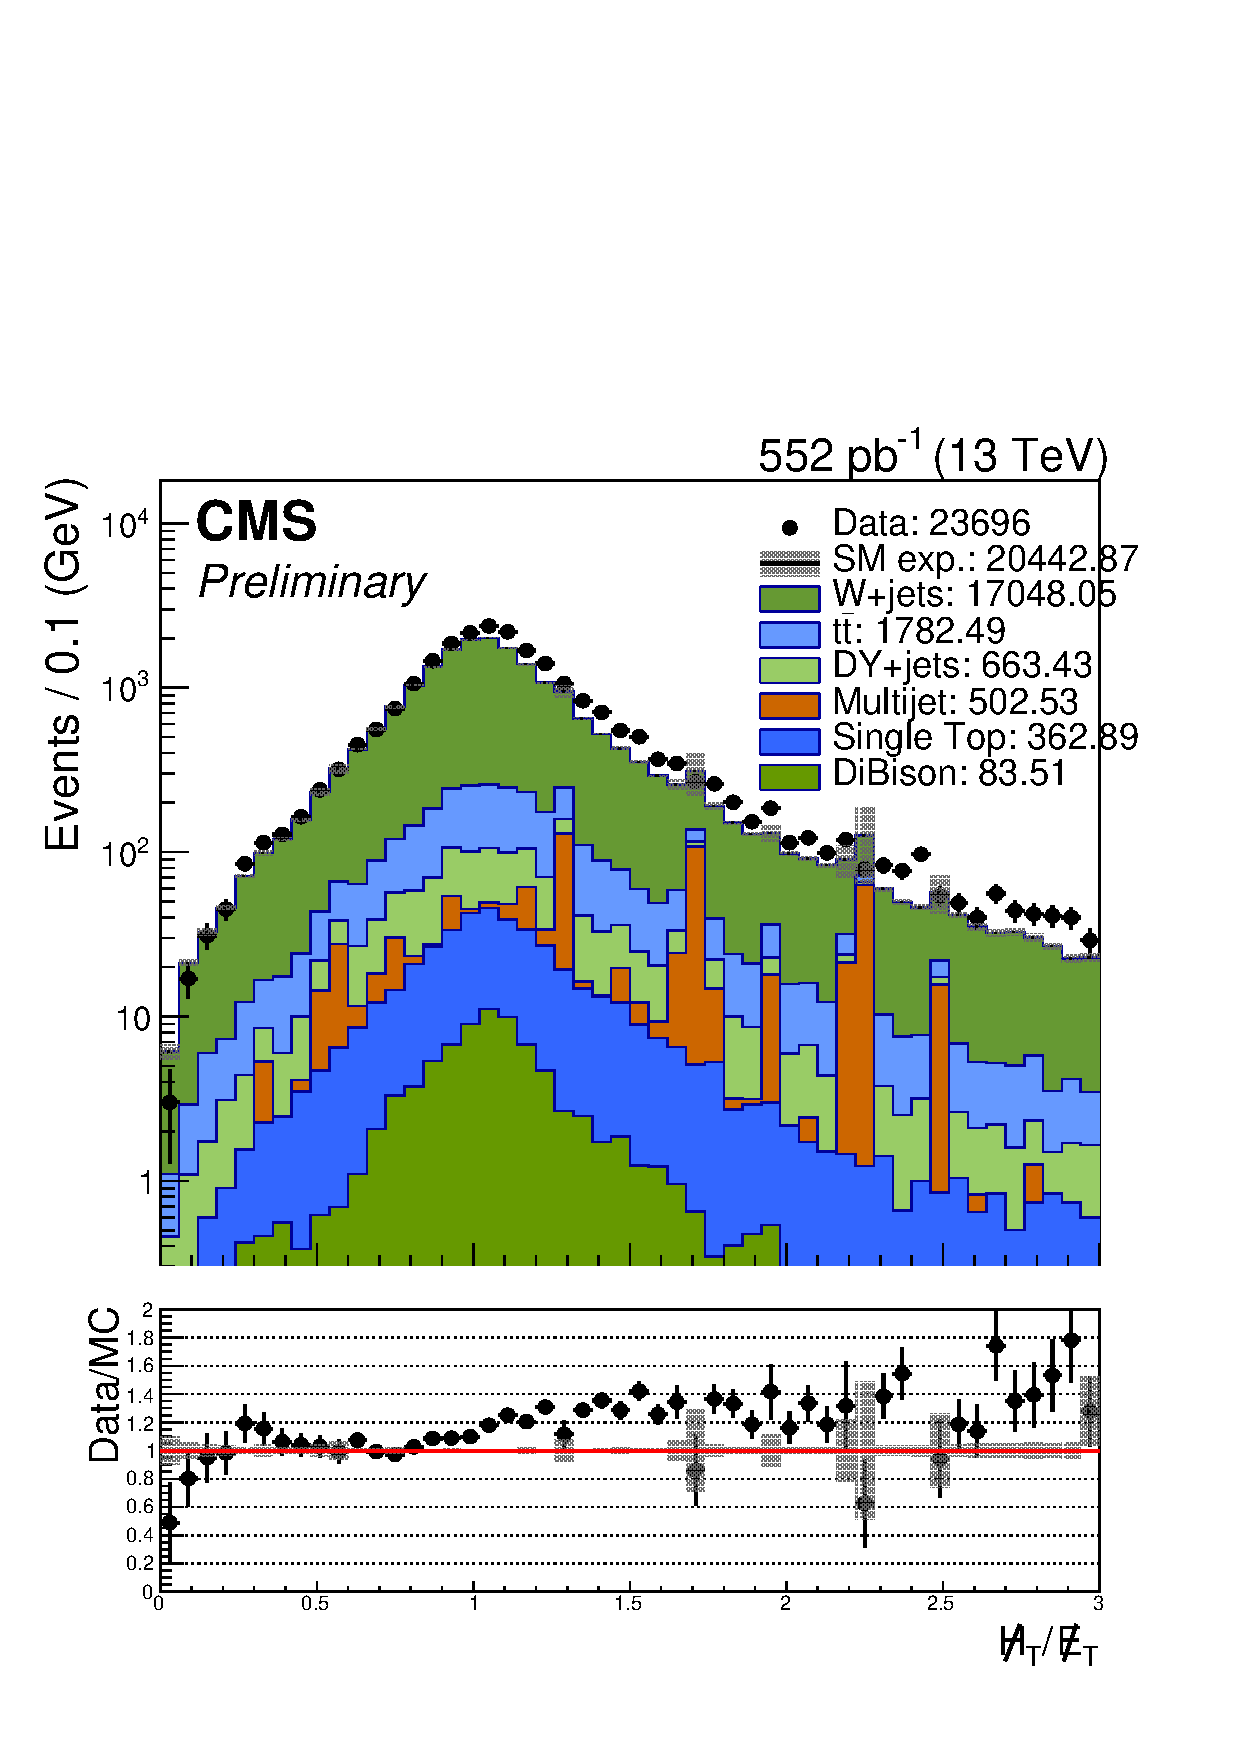
\includegraphics[width=0.31\textwidth]{figures/sidebandCorr/mhtDivMet_NMinusOne_MHTOverMET_WJets}
  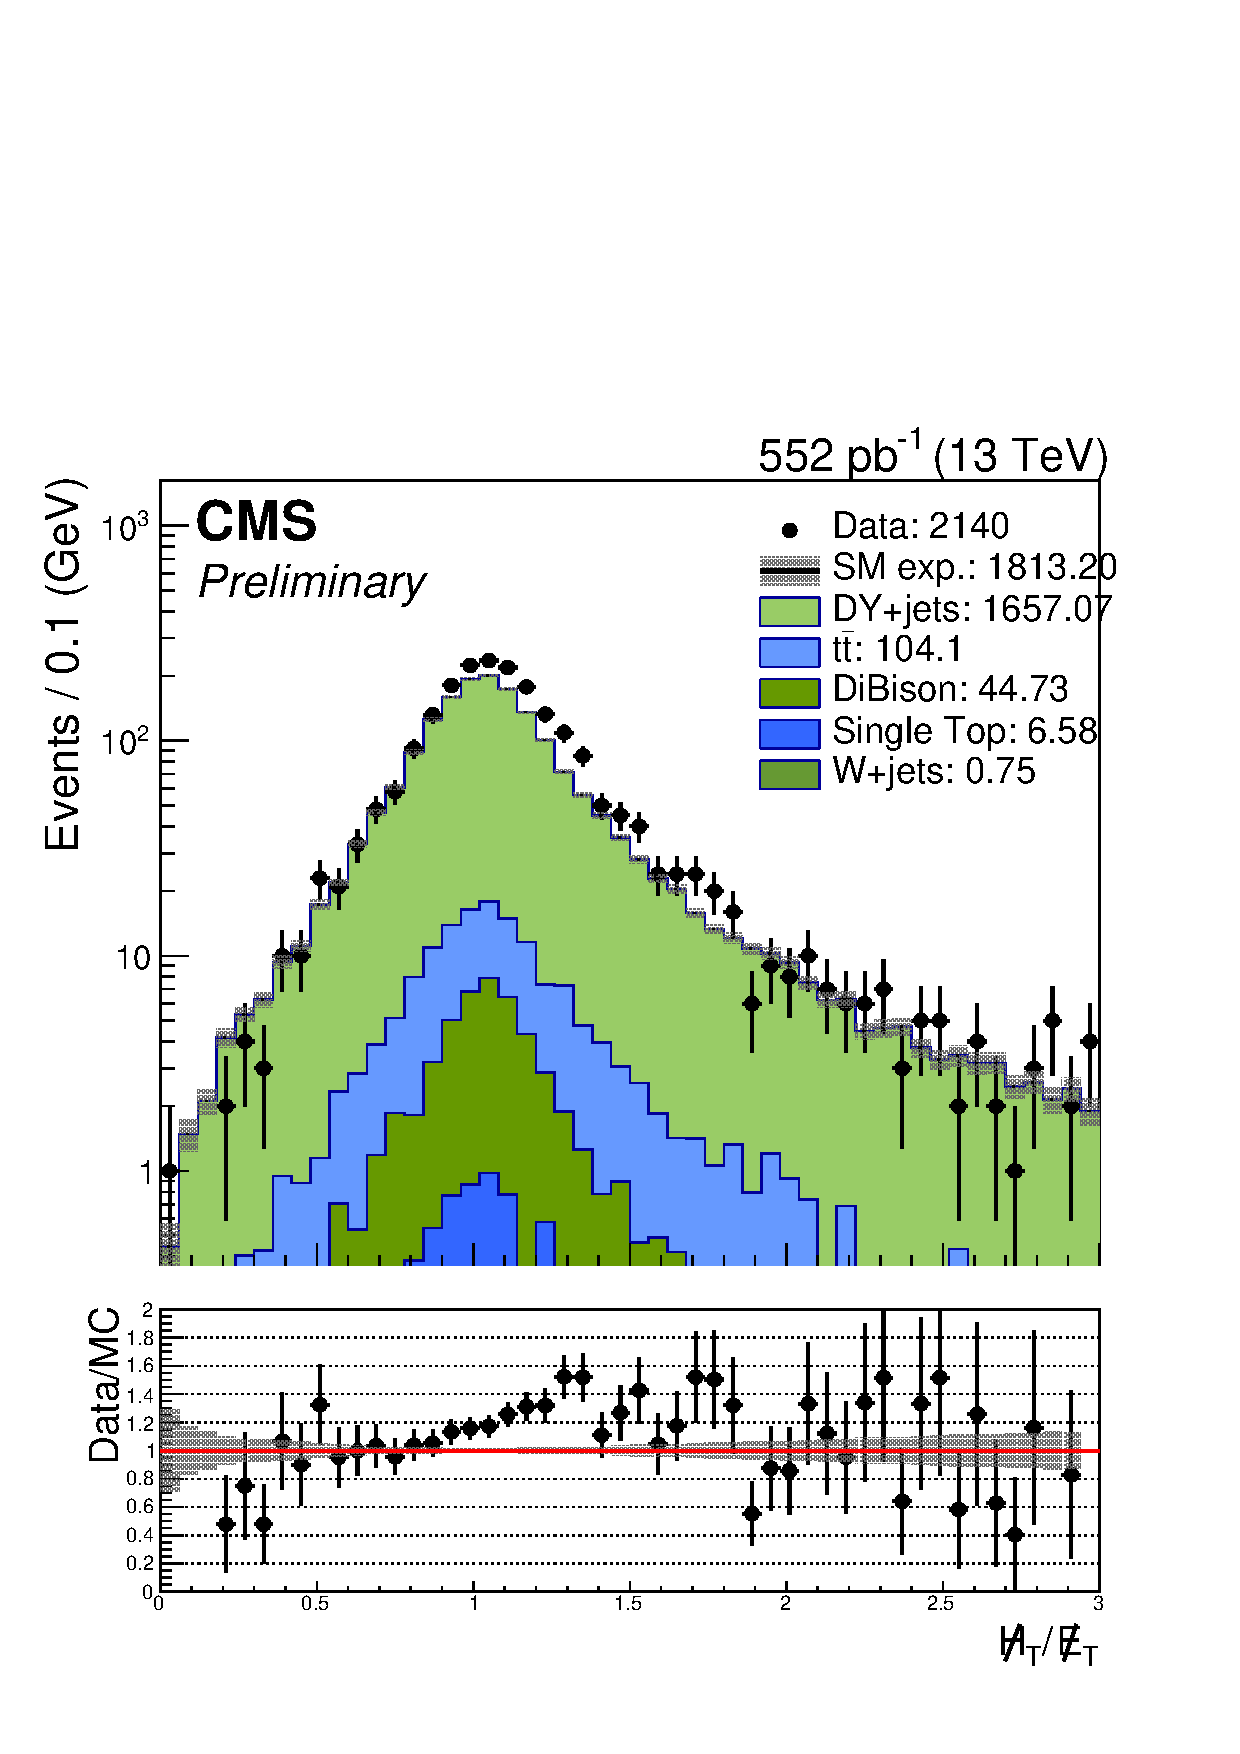
\includegraphics[width=0.31\textwidth]{figures/sidebandCorr/mhtDivMet_NMinusOne_MHTOverMET_DYJetsToLL}
  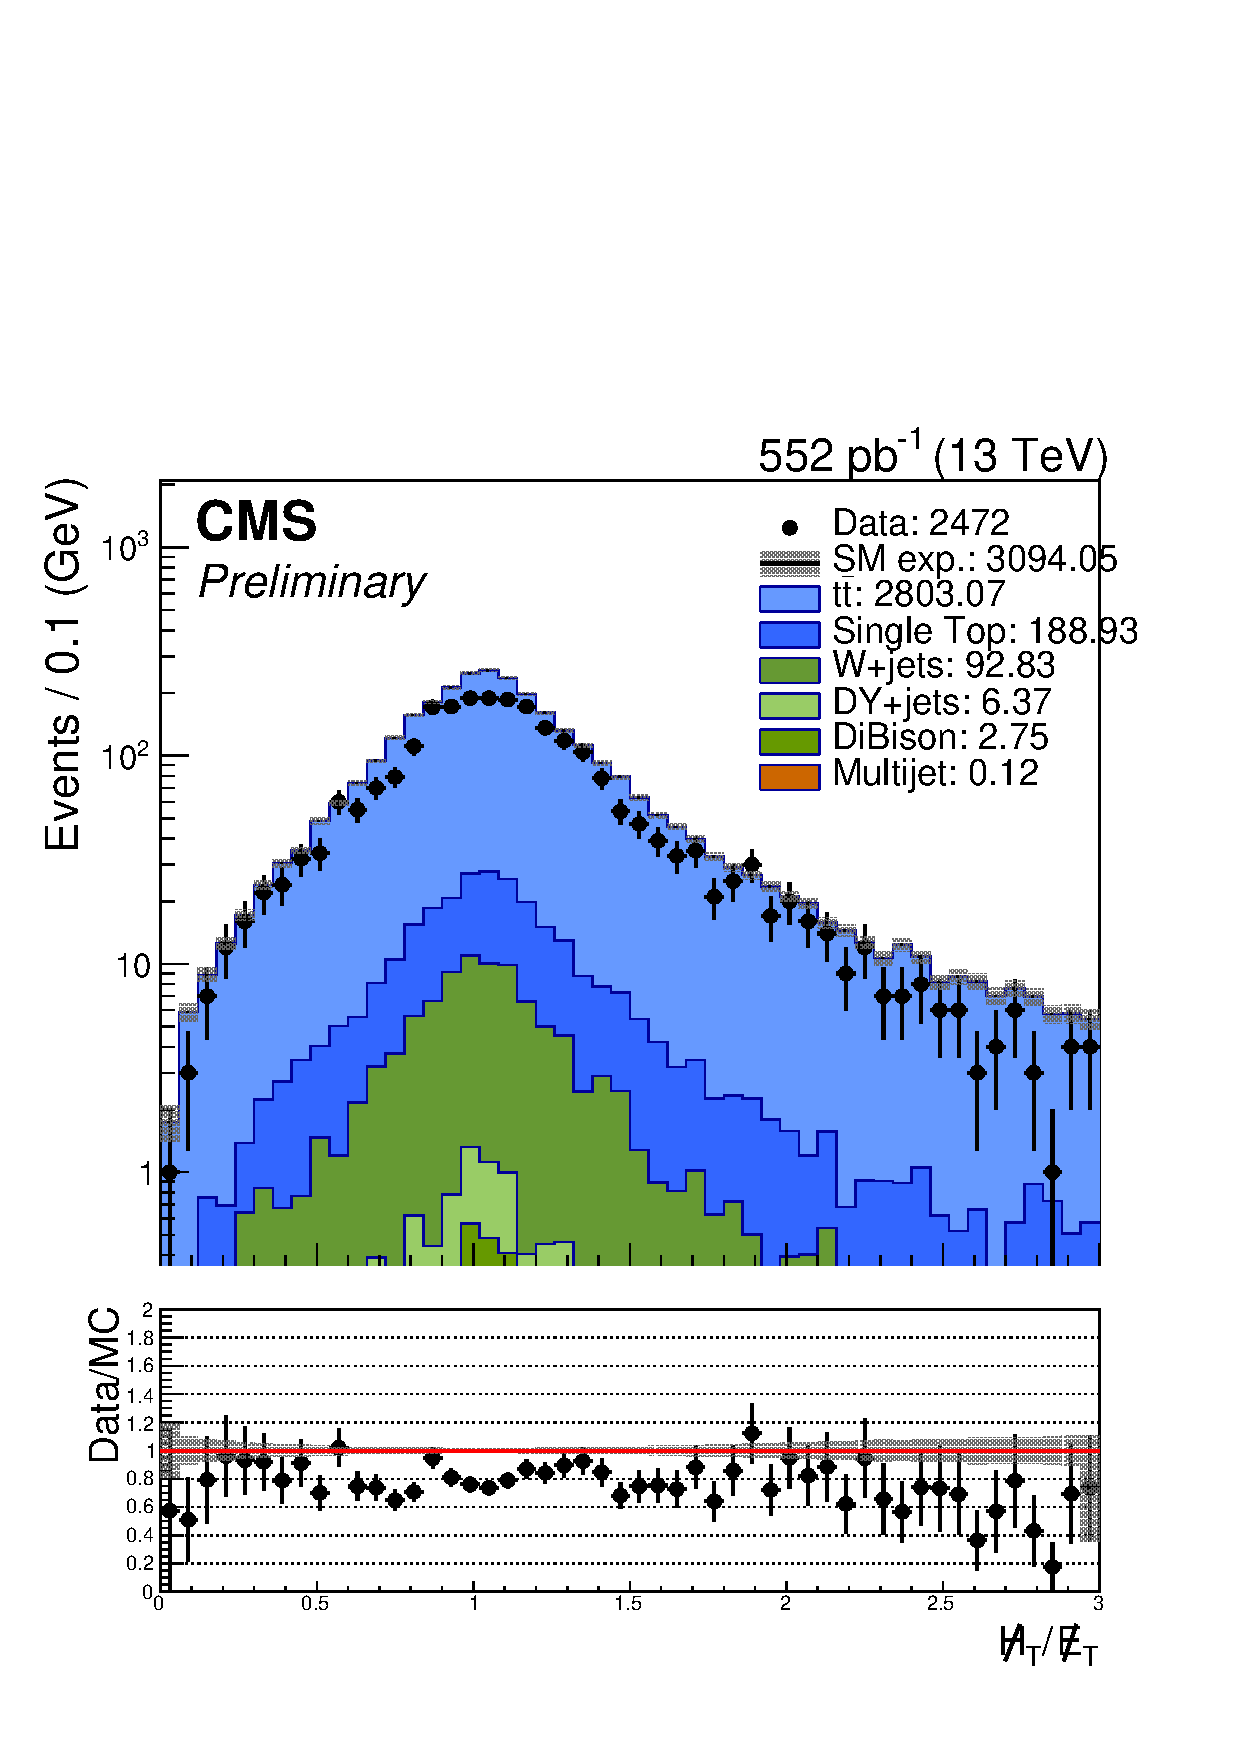
\includegraphics[width=0.31\textwidth]{figures/sidebandCorr/mhtDivMet_NMinusOne_MHTOverMET_TTJets}
  \caption{The ``N-1'' distribution of \mhtmet for the \wj (left), \zj (center) and \ttj (right) selection.}
  \label{fig:w_z_tt_MHTOverMETsideband}
\end{figure}

Given these features of the MC modelling, no conclusive correction is derived from the following studies. 
However, a preliminary investigation on the \scalht dependence of MC corrections is presented, 
with the aim of repeating it in the near future, where a better understanding of the detector will be available. 

In Fig.~\ref{fig:sfVsHt}, the correction factor derived from the \mhtmet sideband is extracted in coarse bins in \scalht for the 3 processes. 
Since the analysis is sensitive to relative corrections rather than absolute ones, the 3 ratios of correction factors 
are showed in Fig.~\ref{fig:double_ratios}. They are compatible with flat within the statistical uncertainties. 
Therefore any \scalht dependence approximately cancels out in the ratio of transfer factors, thus any correction would have a negligible impact. \\
For an inclusive correction, as stated previously, a better understanding of detector effects is required and thus this study is postponed. 

\begin{figure}[!h]
  \centering
  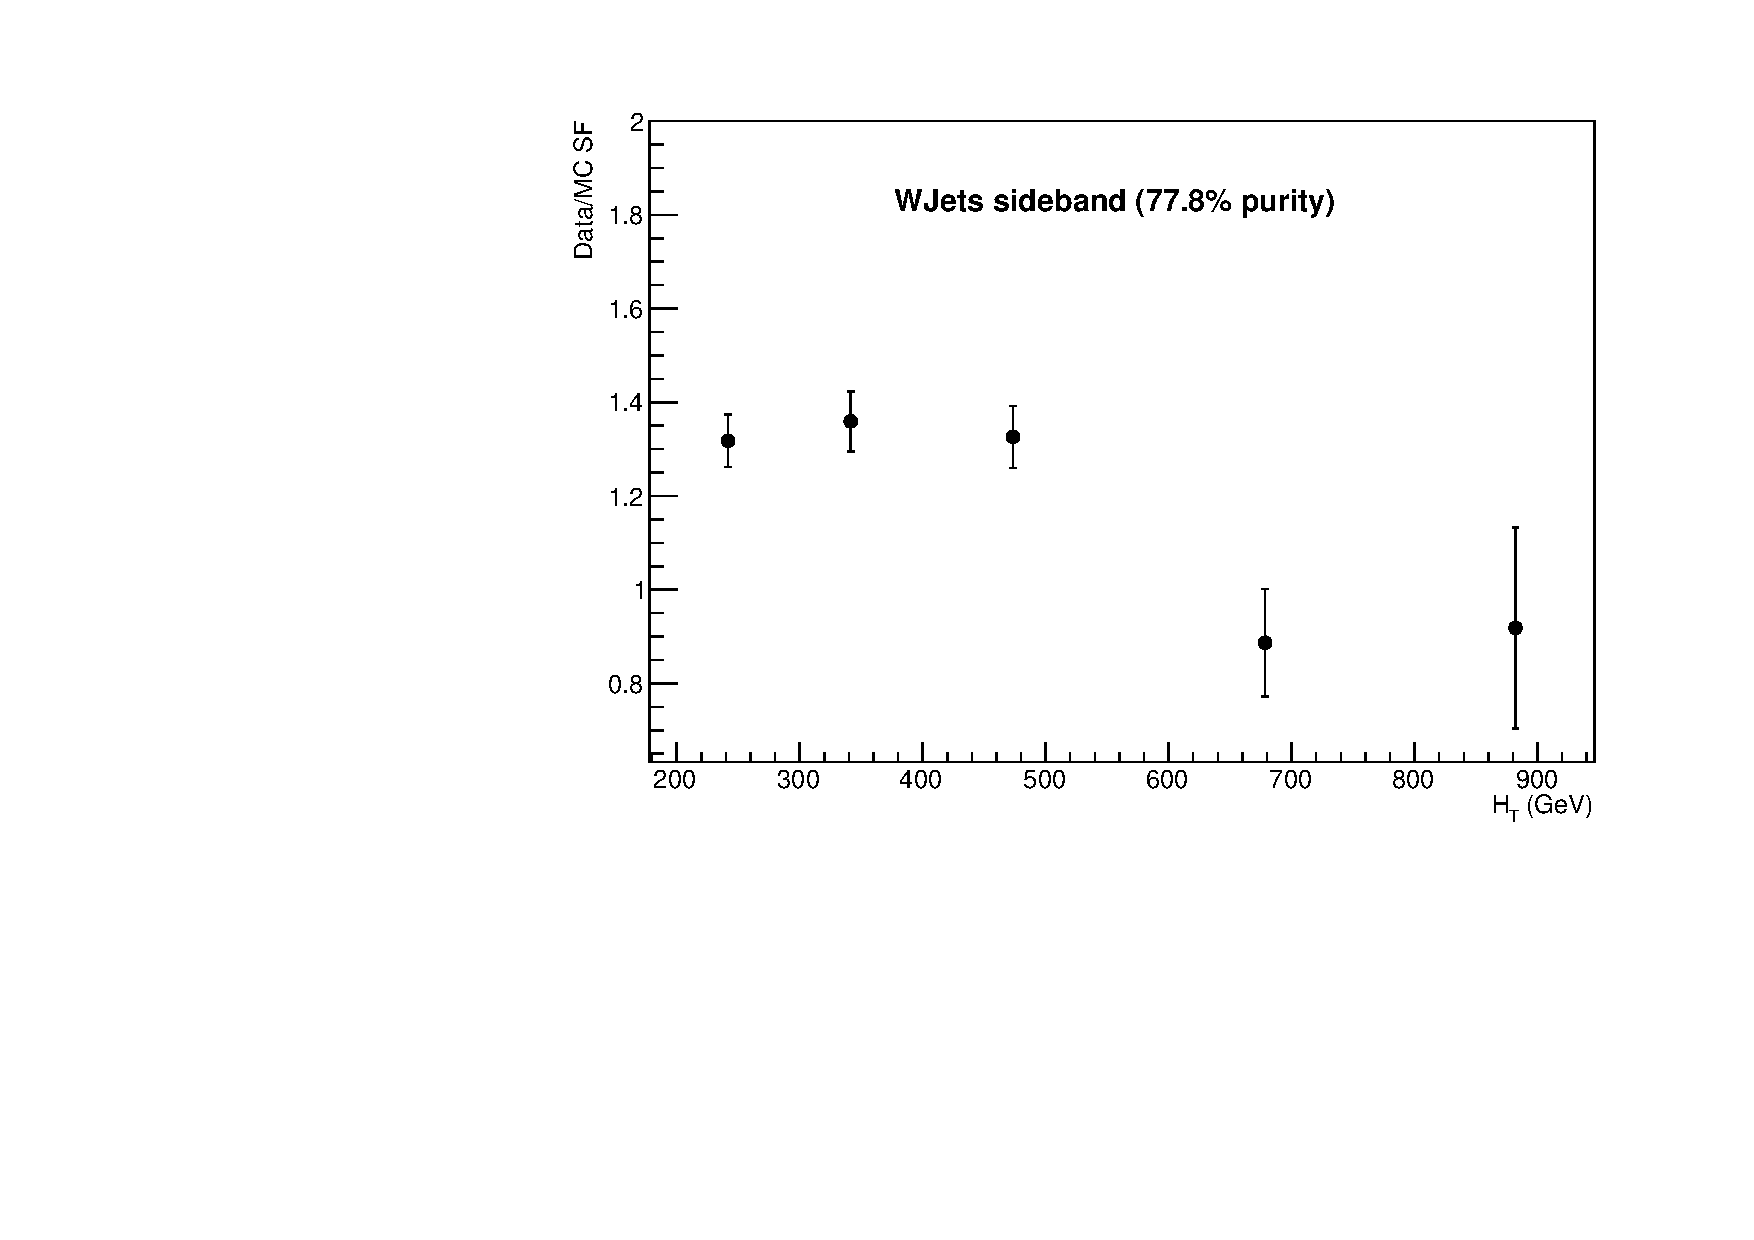
\includegraphics[width=0.31\textwidth]{figures/sidebandCorr/SFvsHT_MHTOverMET_WJets}
  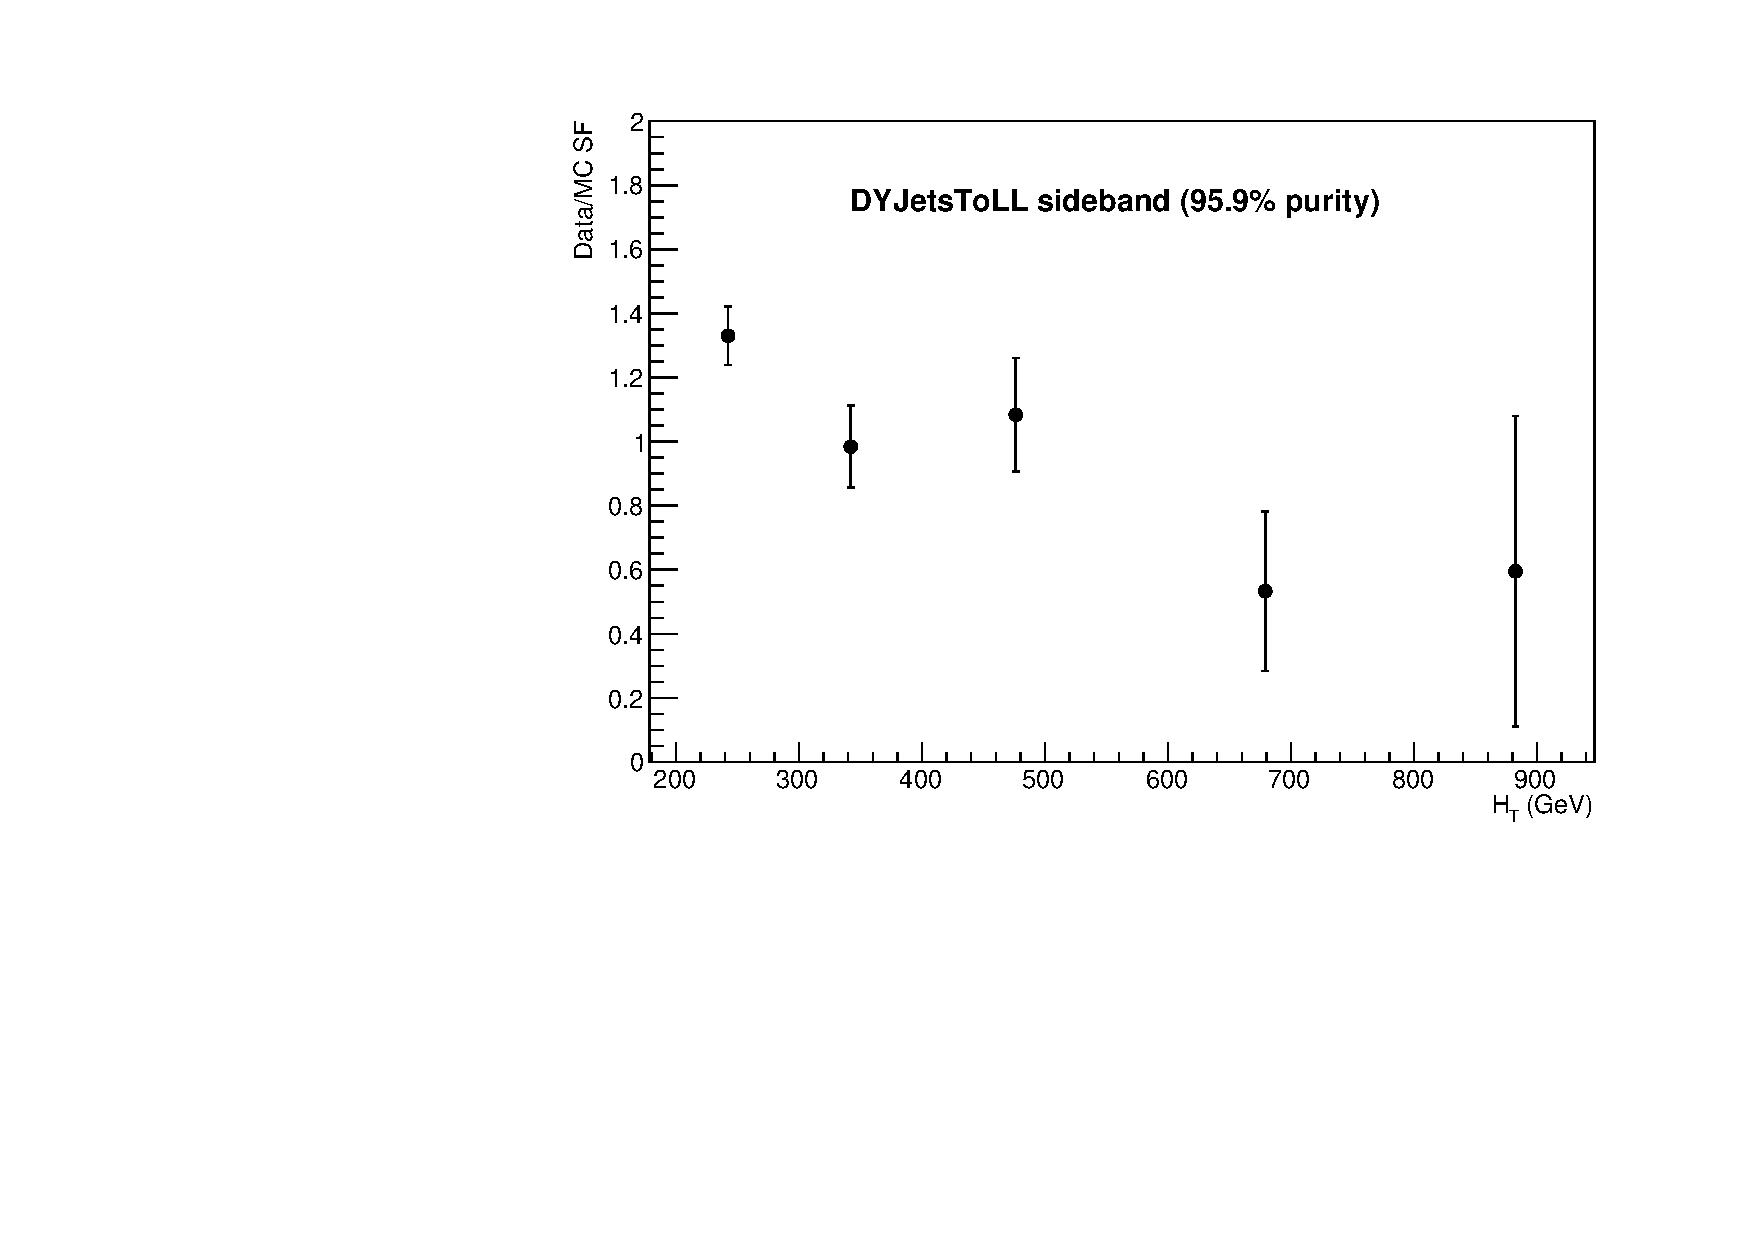
\includegraphics[width=0.31\textwidth]{figures/sidebandCorr/SFvsHT_MHTOverMET_DYJetsToLL}
  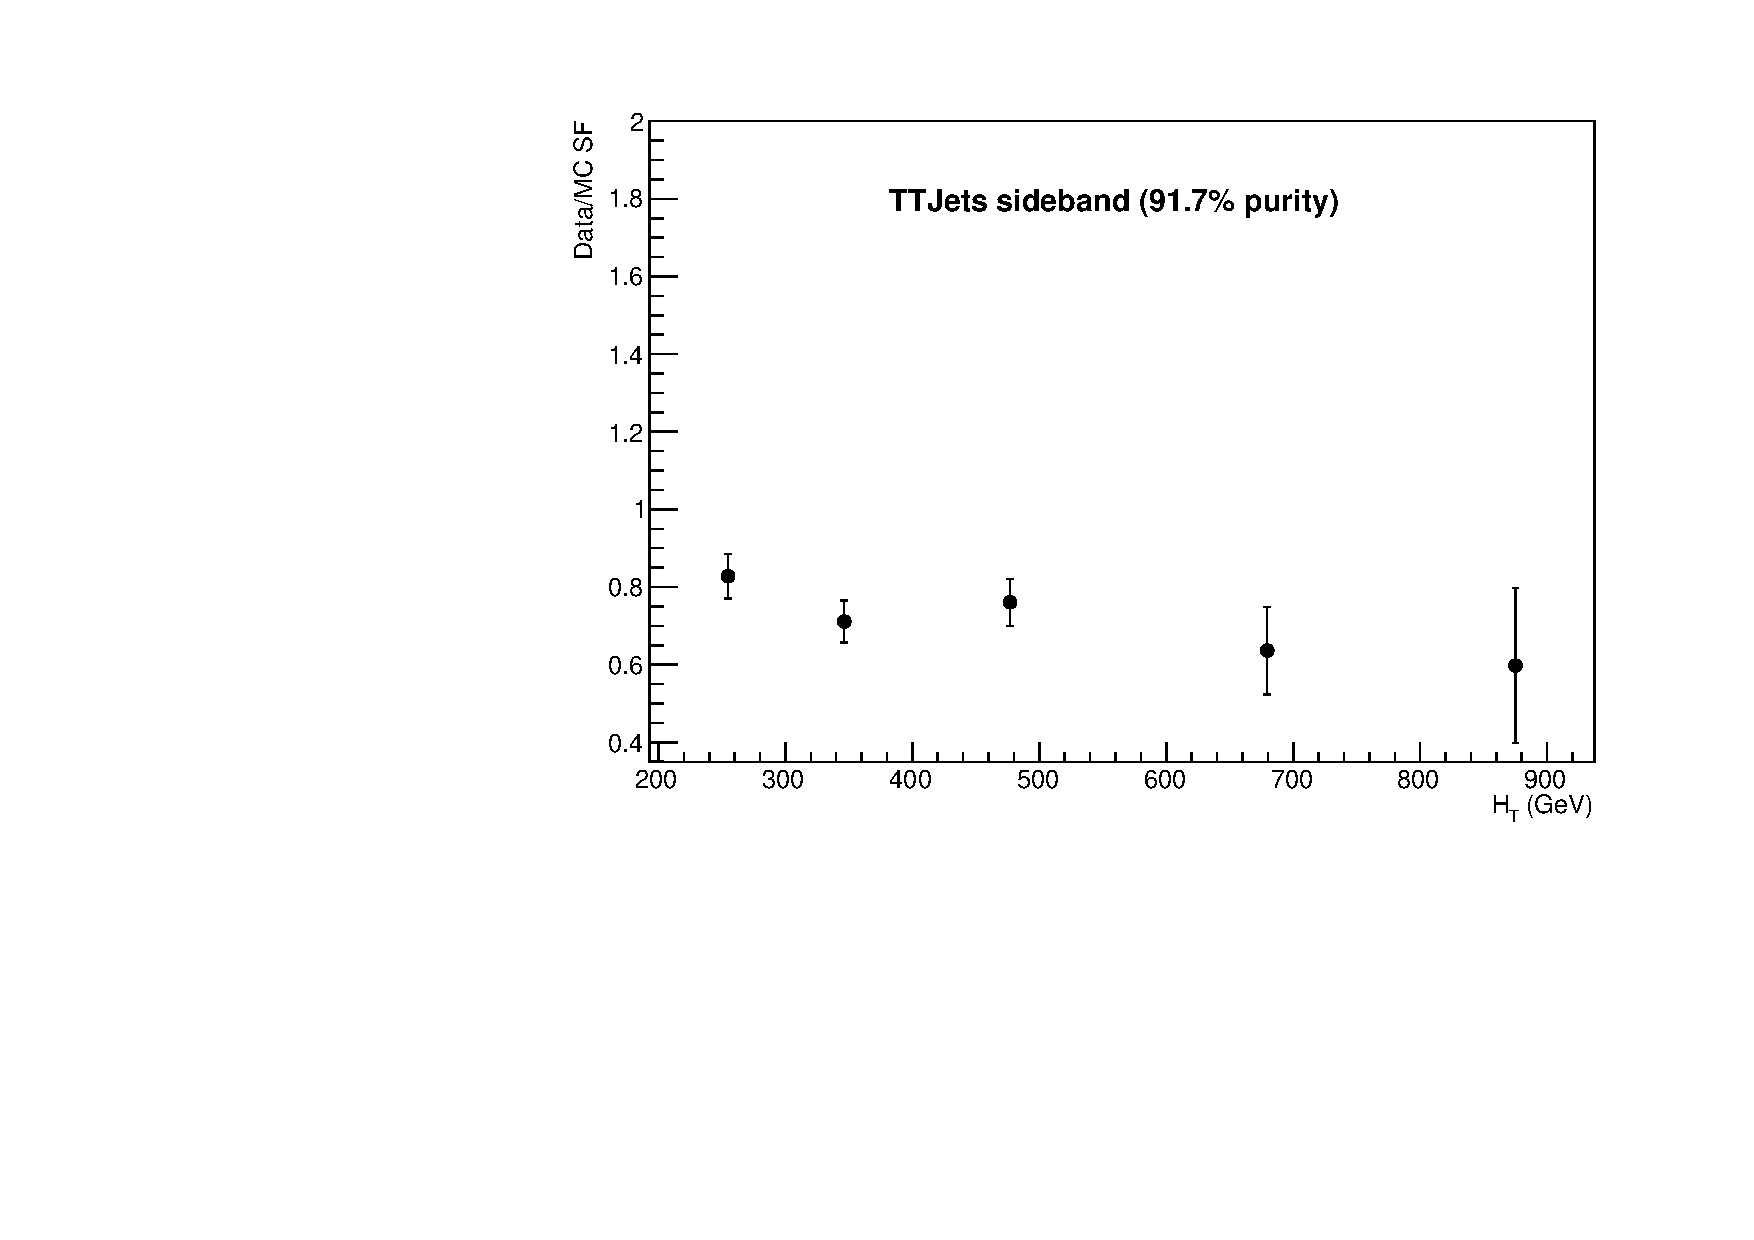
\includegraphics[width=0.31\textwidth]{figures/sidebandCorr/SFvsHT_MHTOverMET_TTJets}
  \caption{The correction factor as a function of \scalht for the \wj (left), \zj (center) and \ttj (right) selection.}
  \label{fig:sfVsHt}
\end{figure}

\begin{figure}[!h]
  \centering
  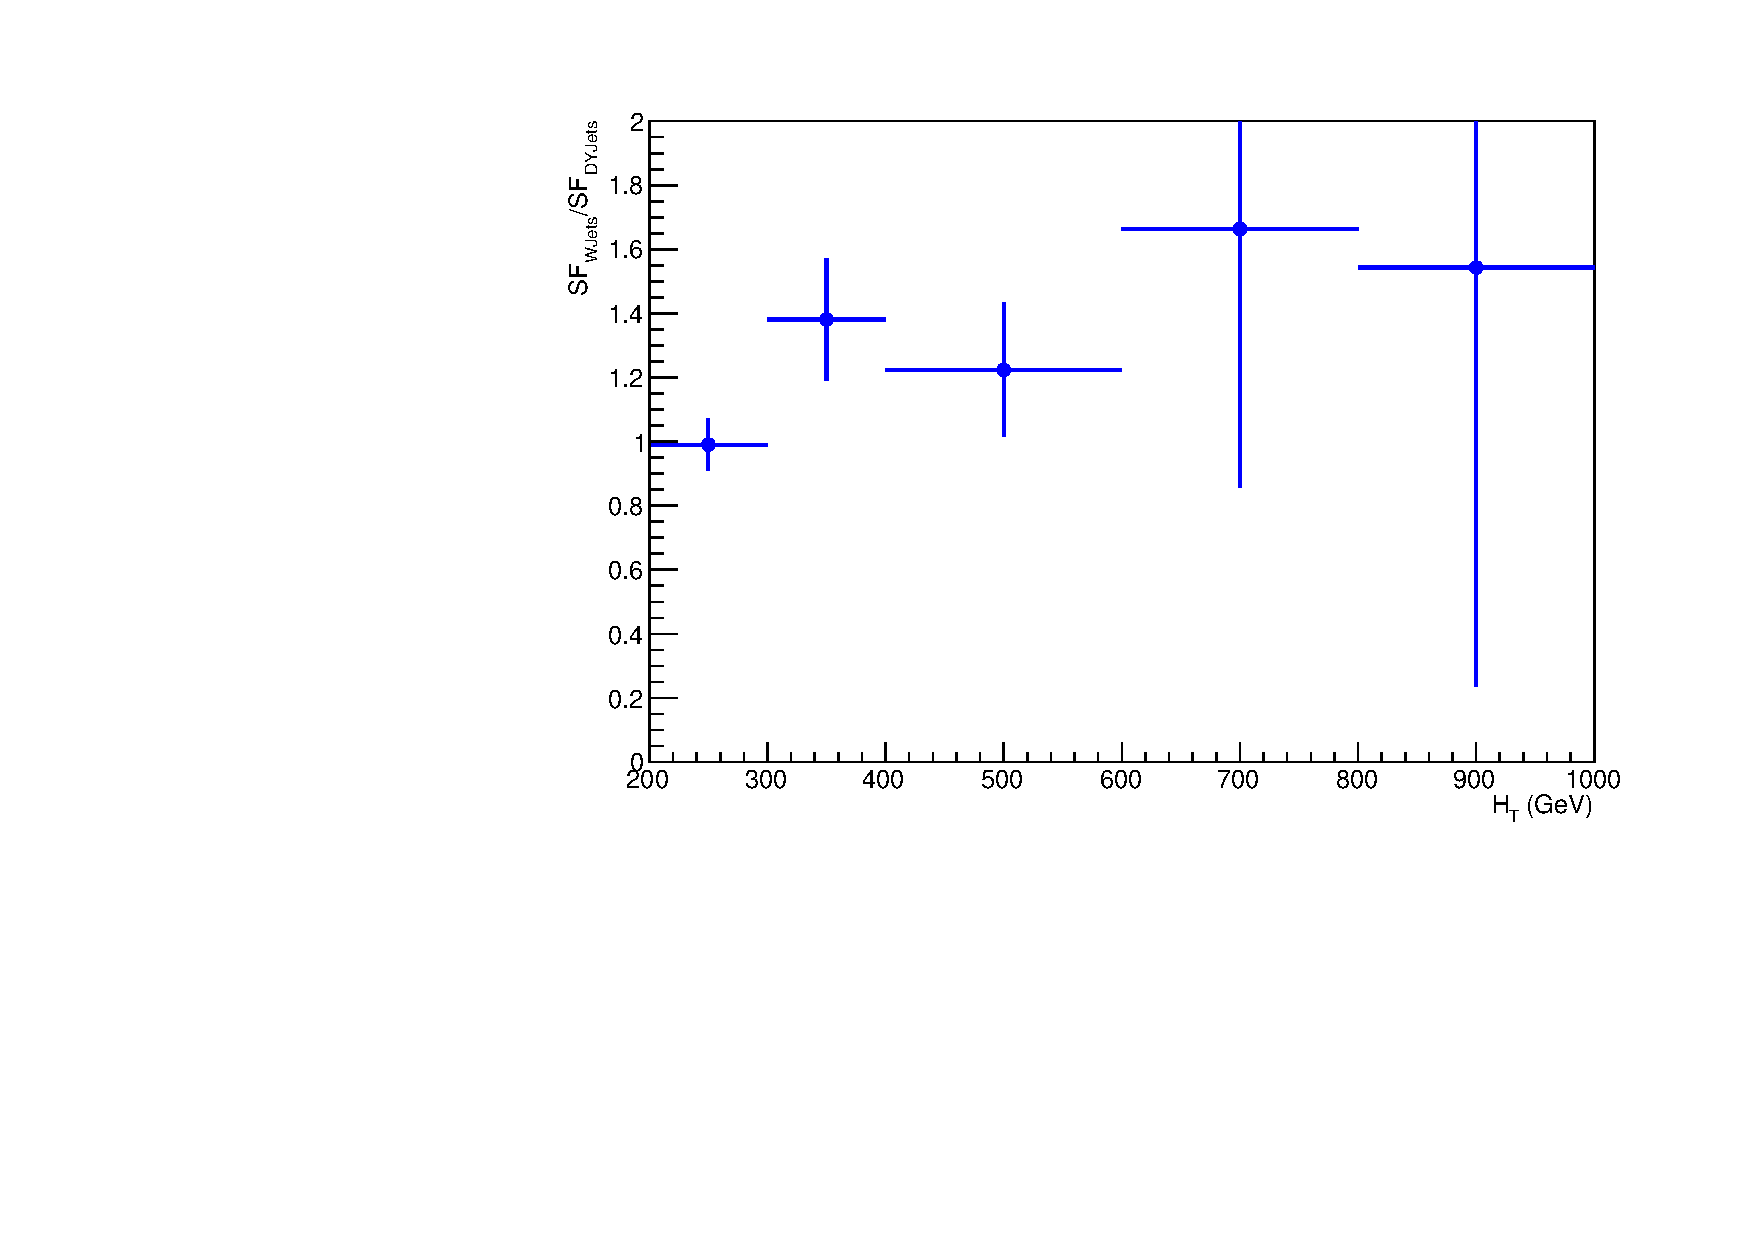
\includegraphics[width=0.31\textwidth]{figures/sidebandCorr/SFDR_w_z}
  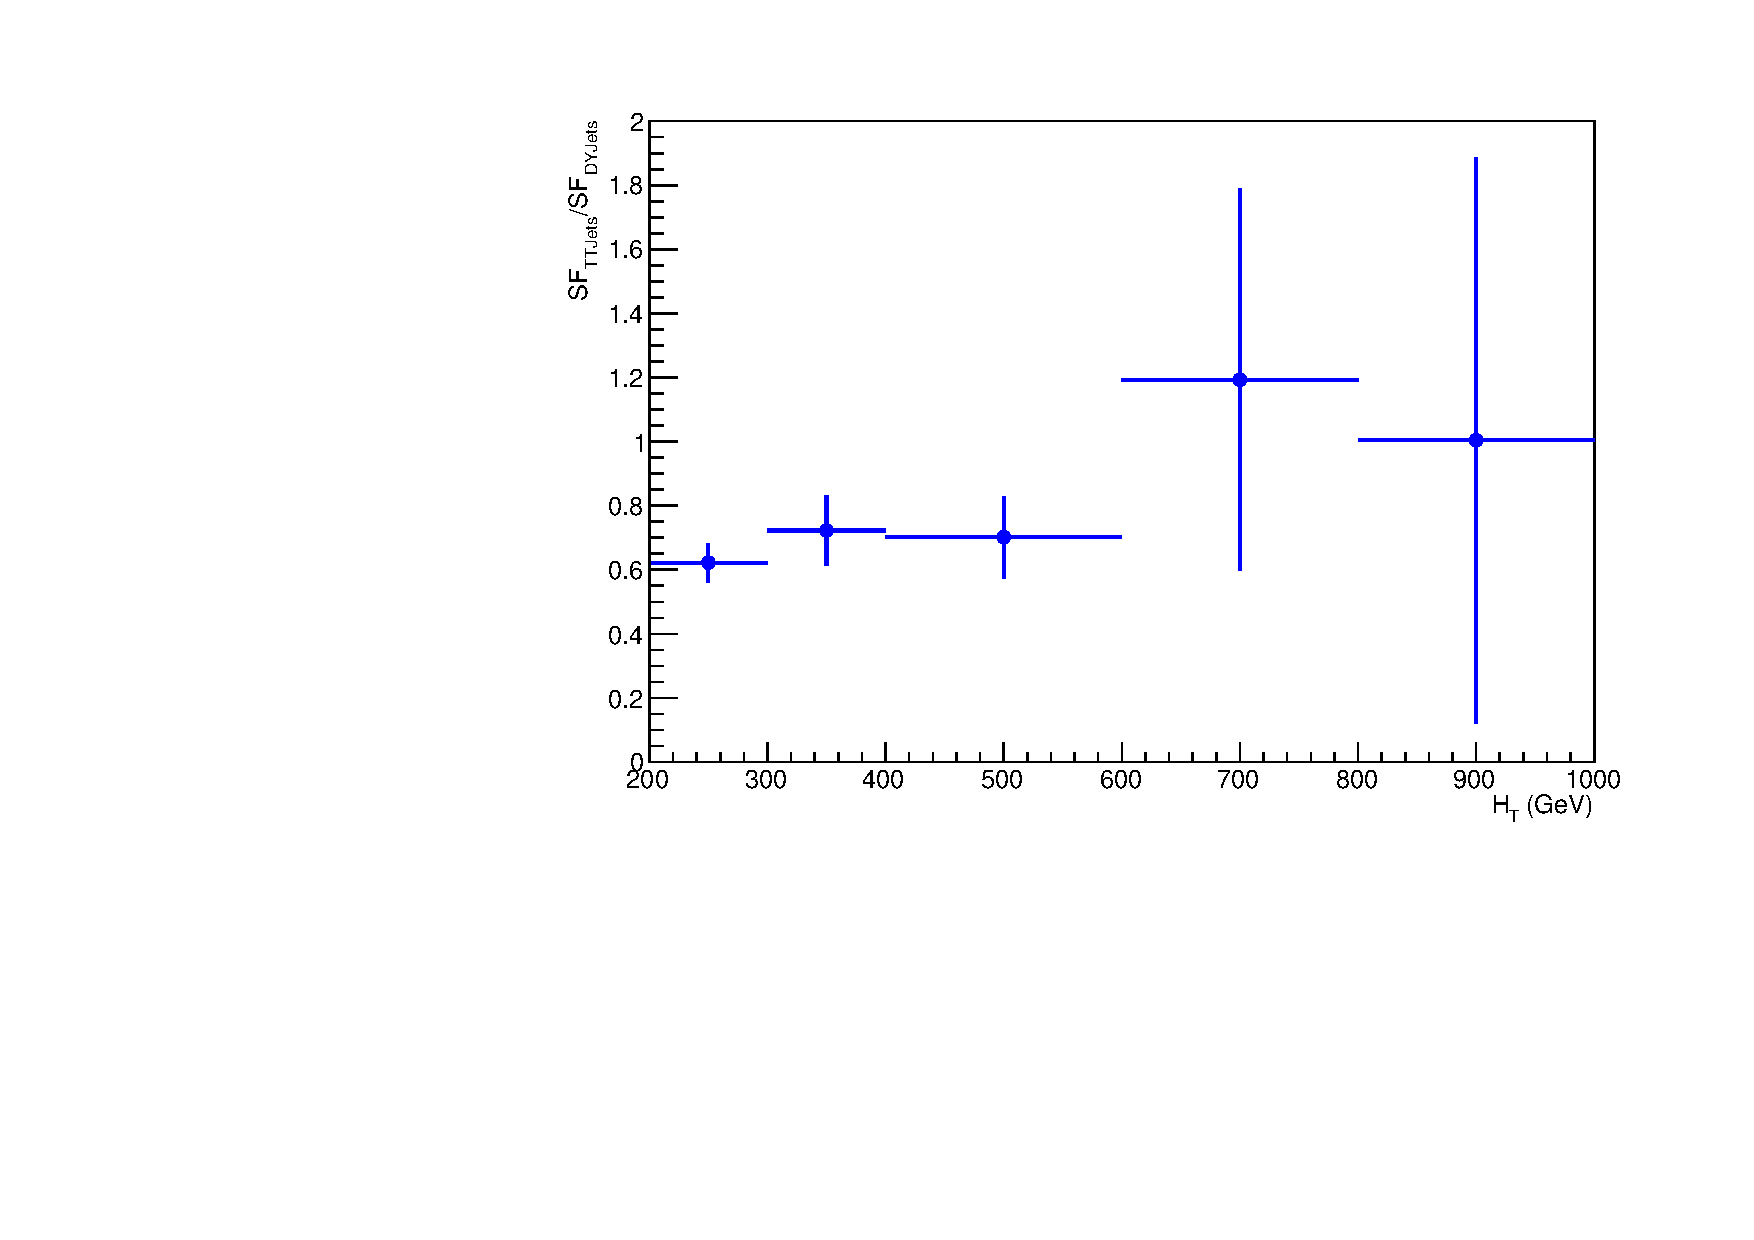
\includegraphics[width=0.31\textwidth]{figures/sidebandCorr/SFDR_tt_z}
  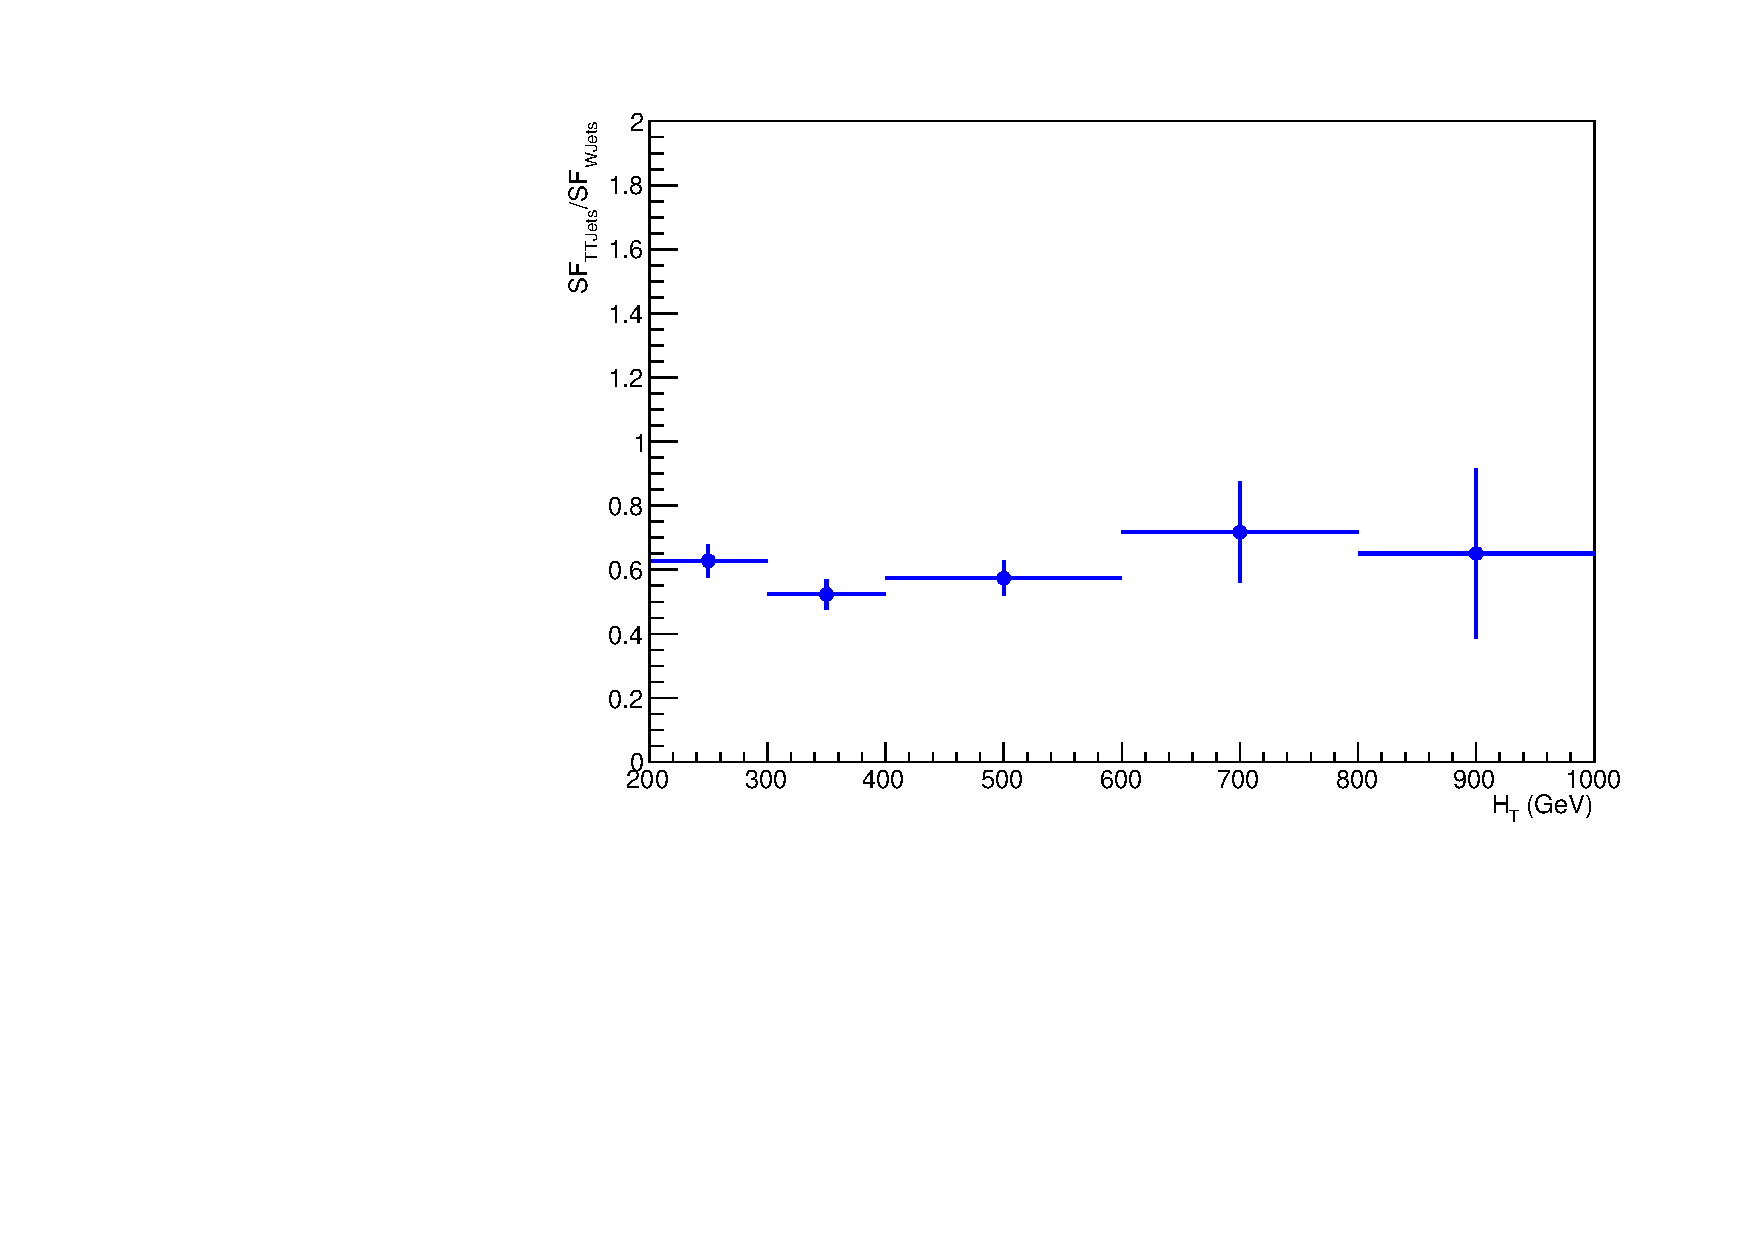
\includegraphics[width=0.31\textwidth]{figures/sidebandCorr/SFDR_tt_w}
  \caption{The ratio of correction factors as a function of \scalht: \wj/\zj (left), \ttj/\zj (center) and \ttj/\wj (right).}
  \label{fig:double_ratios}
\end{figure}

